\documentclass[11pt]{article}
\usepackage{theme}
\usepackage{shortcuts}
% Document parameters
% Document title
\title{Assignment 2 (ML for TS) - MVA}
\author{
Firstname Lastname \email{youremail1@mail.com} \\ % student 1
Firstname Lastname \email{youremail2@mail.com} % student 2
}

\begin{document}
\maketitle

\section{Introduction}

\paragraph{Objective.} The goal is to better understand the properties of AR and MA processes and do signal denoising with sparse coding.

\paragraph{Warning and advice.} 
\begin{itemize}
    \item Use code from the tutorials as well as from other sources. Do not code yourself well-known procedures (e.g., cross-validation or k-means); use an existing implementation. 
    \item The associated notebook contains some hints and several helper functions.
    \item Be concise. Answers are not expected to be longer than a few sentences (omitting calculations).
\end{itemize}



\paragraph{Instructions.}
\begin{itemize}
    \item Fill in your names and emails at the top of the document.
    \item Hand in your report (one per pair of students) by Monday 2\textsuperscript{nd} December 11:59 PM.
    \item Rename your report and notebook as follows:\\ \texttt{FirstnameLastname1\_FirstnameLastname1.pdf} and\\ \texttt{FirstnameLastname2\_FirstnameLastname2.ipynb}.\\
    For instance, \texttt{LaurentOudre\_CharlesTruong.pdf}.
    \item Upload your report (PDF file) and notebook (IPYNB file) using this link: \href{https://docs.google.com/forms/d/e/1FAIpQLSfCqMXSDU9jZJbYUMmeLCXbVeckZYNiDpPl4hRUwcJ2cBHQMw/viewform?usp=sf_link}{https://docs.google.com/forms/d/e/1FAIpQLSfCqMXSDU9jZJbYUMmeLCXbVeckZYNiDpPl4hRUwcJ2cBHQMw/viewform?usp=sf\_link}.
\end{itemize}


\section{General questions}

A time series $\{y_t\}_t$ is a single realisation of a random process $\{Y_t\}_t$ defined on the probability space $(\Omega, \mathcal{F}, P)$, i.e. $y_t = Y_t(w)$ for a given $w\in\Omega$.
In classical statistics, several independent realizations are often needed to obtain a ``good'' estimate (meaning consistent) of the parameters of the process.
However, thanks to a stationarity hypothesis and a "short-memory" hypothesis, it is still possible to make ``good'' estimates.
The following question illustrates this fact.

\begin{exercise}
An estimator $\hat{\theta}_n$ is consistent if it converges in probability when the number $n$ of samples grows to $\infty$ to the true value $\theta\in\mathbb{R}$ of a parameter, i.e. $\hat{\theta}_n \xrightarrow{\mathcal{D}} \theta$.

\begin{itemize}
    \item Recall the rate of convergence of the sample mean for i.i.d.\ random variables with finite variance.
    \item Let $\{Y_t\}_{t\geq 1}$ a wide-sense stationary process such that $\sum_k |\gamma (k)| < +\infty$. 
    Show that the sample mean $\bar{Y}_n = (Y_1+\dots+Y_n)/n$ is consistent and enjoys the same rate of convergence as the i.i.d.\ case. (Hint: bound $\mathbb{E}[(\bar{Y}_n-\mu)^2]$ with the $\gamma (k)$ and recall that convergence in $L_2$ implies convergence in probability.)
\end{itemize}

\end{exercise}

\begin{solution}  % ANSWER HERE

\[
\widehat{\theta}_n = \frac{1}{n} \sum_{i=1}^n \theta_i
\]

\[
\mathbb{E} \left[ \left( \widehat{\theta}_n - \theta \right)^2 \right] = \text{Var}(\widehat{\theta}_n)
\]

\[
= \frac{1}{n} \text{Var}(\theta_1)
\]

Since the \(L_2\)-convergence implies the \(P\)-convergence, the convergence rate of \(\widehat{\theta}_n\) is:

\[
\frac{1}{n}.
\]

\subsection*{2.}

\[
\mathbb{E} \left[ \left( \overline{Y}_n - \mu \right)^2 \right] = \mathbb{E} \left[ \left( \frac{1}{n} \sum_{i=1}^n (Y_i - \mu) \right)^2 \right]
\]

\[
= \mathbb{E} \left[ \frac{1}{n^2} \sum_{i=1}^n (Y_i - \mu) \sum_{j=1}^n (Y_j - \mu) \right]
\]

\[
= \frac{1}{n^2} \sum_{i=1}^n \sum_{j=1}^n \mathbb{E} \left[ (Y_i - \mu)(Y_j - \mu) \right]
\]

\[
= \frac{1}{n^2} \sum_{i=1}^n \sum_{j=1}^n \gamma(j - i)
\]

\[
\leq \frac{1}{n^2} \sum_{i=1}^n \sum_{j \in \mathbb{Z}} |\gamma(j)|
\]

\[
\leq \frac{1}{n} \sum_{j \in \mathbb{Z}} |\gamma(j)|.
\]

Again, we can conclude that the convergence rate of \(\overline{Y}_n\) is:

\[
\frac{1}{n}.
\]



\end{solution}


\newpage
\section{AR and MA processes}

\begin{exercise}[subtitle=Infinite order moving average MA($\infty$)]
Let $\{Y_t\}_{t\geq 0}$ be a random process defined by
\begin{equation}\label{eq:ma-inf}
    Y_t = \varepsilon_t + \psi_1 \varepsilon_{t-1} + \psi_2 \varepsilon_{t-2} + \dots = \sum_{k=0}^{\infty} \psi_k\varepsilon_{t-k}
\end{equation}
where $(\psi_k)_{k\geq0} \subset \mathbb{R}$ ($\psi=1$) are square summable, \ie $\sum_k \psi_k^2 < \infty$ and $\{\varepsilon_t\}_t$ is a zero mean white noise of variance $\sigma_\varepsilon^2$.
(Here, the infinite sum of random variables is the limit in $L_2$ of the partial sums.)
\begin{itemize}
    \item Derive $\mathbb{E}(Y_t)$ and $\mathbb{E}(Y_t Y_{t-k})$. Is this process weakly stationary?
    \item Show that the power spectrum of $\{Y_t\}_{t}$ is $S(f) = \sigma_\varepsilon^2 |\phi(e^{-2\pi\iu f})|^2$ where $\phi(z) = \sum_j \psi_j z^j$. (Assume a sampling frequency of 1 Hz.)
\end{itemize}

The process $\{Y_t\}_{t}$ is a moving average of infinite order.
Wold's theorem states that any weakly stationary process can be written as the sum of the deterministic process and a stochastic process which has the form~\eqref{eq:ma-inf}.

\end{exercise}

\begin{solution}  % ANSWER HERE

\end{solution}

\newpage
\begin{exercise}[subtitle=AR(2) process]
Let $\{Y_t\}_{t\geq 1}$ be an AR(2) process, i.e.
\begin{equation}
    Y_t = \phi_1 Y_{t-1} + \phi_2 Y_{t-2} + \varepsilon_t
\end{equation}
with $\phi_1, \phi_2\in\mathbb{R}$.
The associated characteristic polynomial is $\phi(z):=1-\phi_1 z - \phi_2 z^2$.
Assume that $\phi$ has two distinct roots (possibly complex) $r_1$ and $r_2$ such that $|r_i|>1$.
Properties on the roots of this polynomial drive the behavior of this process.


\begin{itemize}
    \item Express the autocovariance coefficients $\gamma(\tau)$ using the roots $r_1$ and $r_2$.
    \item Figure~\ref{fig:q-ar-2-corr} shows the correlograms of two different AR(2) processes. Can you tell which one has complex roots and which one has real roots?
    \item Express the power spectrum $S(f)$ (assume the sampling frequency is 1 Hz) using $\phi(\cdot)$.
    \item Choose $\phi_1$ and $\phi_2$ such that the characteristic polynomial has two complex conjugate roots of norm $r=1.05$ and phase $\theta=2\pi/6$. Simulate the process $\{Y_t\}_t$ (with $n=2000$) and display the signal and the periodogram (use a smooth estimator) on Figure~\ref{fig:q-ar-2}. What do you observe?
\end{itemize}


\begin{figure}
    \centering
    \begin{minipage}[t]{0.45\textwidth}
    \centerline{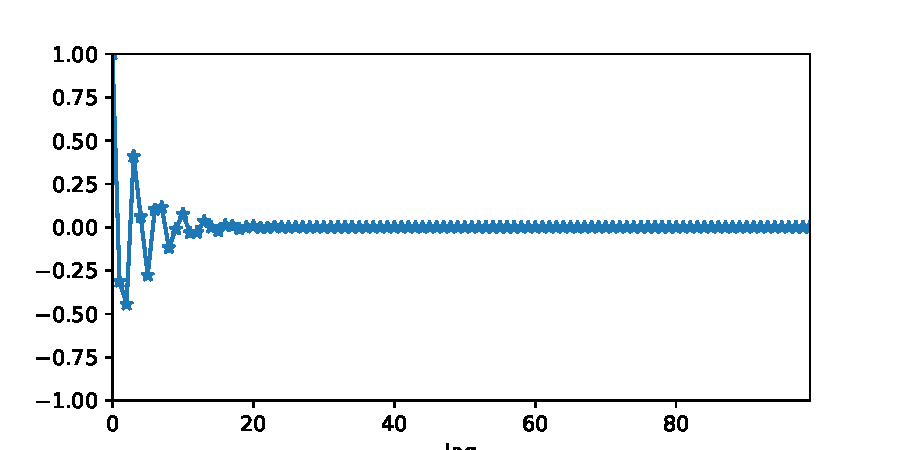
\includegraphics[width=\textwidth]{images/acf1.pdf}}
    \centerline{Correlogram of the first AR(2)}
    \end{minipage}
    \hfill
    \begin{minipage}[t]{0.45\textwidth}    \centerline{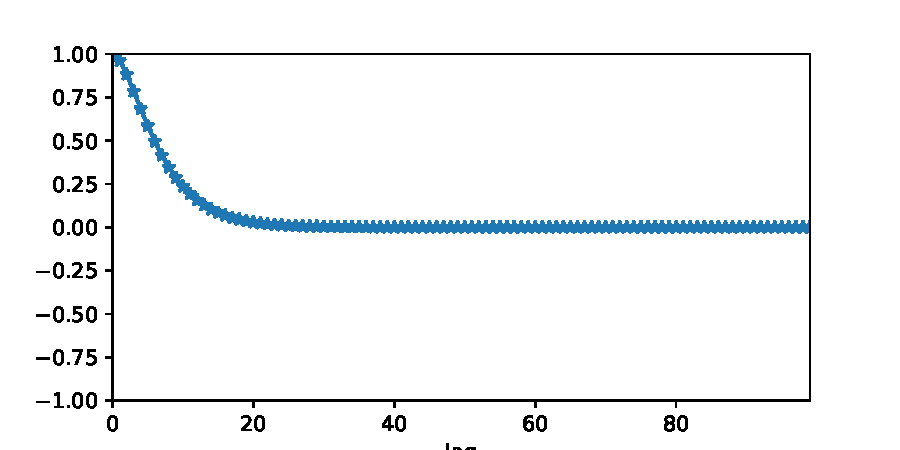
\includegraphics[width=\textwidth]{images/acf2.pdf}}
    \centerline{Correlogram of the second AR(2)}
    \end{minipage}
    \caption{Two AR(2) processes}\label{fig:q-ar-2-corr}
\end{figure}



\end{exercise}

\begin{solution}  % ANSWER HERE

\[
Y_t = \phi_1 Y_{t-1} + \phi_2 Y_{t-2} + \varepsilon_t
\]

\[
\mathbb{E}[Y_t Y_{t-\tau}] = \phi_1 \gamma(\tau-1) + \phi_2 \gamma(\tau-2) + 0
\]

\[
\implies \gamma(\tau) = \phi_1 \gamma(\tau-1) + \phi_2 \gamma(\tau-2)
\]

\subsection*{Suite récurrente d'ordre 2:}
\[
\gamma(\tau) = A r_1^\tau+ B r_2^\tau
\]

\[
\gamma(0) = 1
\]

\[
\gamma(1) = \phi_1 \gamma(0) + \gamma(1) \phi_2
\]

\[
\implies \gamma(1) = \frac{\phi_1}{1 - \phi_2}
\]

\[
\begin{cases}
A + B = 1 \\
Ar_1 + Br_2 = \frac{\phi_1}{1 - \phi_2}
\end{cases}
\]

\[
B = \left( \frac{\phi_1}{1 - \phi_2} - r_1 \right) \cdot \frac{1}{r_2 - r_1}
\]

\[
A = B - 1
\]

Then, the first AR with oscillations correspond to the complex roots and the second AR correspond to the real roots.
\[
S(t) = \sum_{k=0}^{\infty} x(t-kT) e^{-2\pi ktf}
= A * ( \frac{2}{1 - r_1 e^{2i\pi f/f_s}} - 1 ) + B * ( \frac{2}{1 - r_2 e^{2i\pi f/f_s}} - 1 ) 
\]


\begin{figure}
    \centering
    \begin{minipage}[t]{0.45\textwidth}
    \centerline{\includegraphics[width=\textwidth]{example-image-golden}}
    \centerline{Signal}
    \end{minipage}
    \hfill
    \begin{minipage}[t]{0.45\textwidth}    \centerline{\includegraphics[width=\textwidth]{example-image-golden}}
    \centerline{Periodogram}
    \end{minipage}
    \caption{AR(2) process}\label{fig:q-ar-2}
\end{figure}

\begin{figure}
    \centering
    \begin{minipage}[t]{0.45\textwidth}
    \centerline{\includegraphics[width=\textwidth]{}}
    \centerline{Signal}
    \end{minipage}
    \hfill
    \begin{minipage}[t]{0.45\textwidth}    \centerline{\includegraphics[width=\textwidth]{example-image-golden}}
    \centerline{Periodogram}
    \end{minipage}
    \caption{AR(2) process}\label{fig:q-ar-2}
\end{figure}

\end{solution}

\newpage
\section{Sparse coding}

The modulated discrete cosine transform (MDCT) is a signal transformation often used in sound processing applications (for instance, to encode an MP3 file).
A MDCT atom $\phi_{L,k}$ is defined for a length 2L and a frequency localisation $k$ ($k=0,\dots,L-1$) by
\begin{equation}
\forall u=0,\dots,2L-1,\quad\phi_{L,k}[u]=w_{L}[u]\sqrt{\frac{2}{L}} \cos [ \frac{\pi}{L} \left(u+ \frac{L+1}{2}\right) (k+\frac{1}{2}) ]
\end{equation}
where $w_{L}$ is a modulating window given by
\begin{equation}
w_L[u] = \sin \left[{\frac {\pi }{2L}}\left(u+{\frac {1}{2}}\right)\right].
\end{equation}


\begin{exercise}[subtitle=Sparse coding with OMP]
For the signal provided in the notebook, learn a sparse representation with MDCT atoms.
The dictionary is defined as the concatenation of all shifted MDCDT atoms for scales $L$ in $[32, 64, 128, 256, 512, 1024]$.

\begin{itemize}
    \item For the sparse coding, implement the Orthogonal Matching Pursuit (OMP). (Use convolutions to compute the correlation coefficients.)
    \item Display the norm of the successive residuals and the reconstructed signal with 10 atoms.
\end{itemize}

\end{exercise}
\begin{solution}


\begin{figure}
    \centering
    \begin{minipage}[t]{0.45\textwidth}
    \centerline{\includegraphics[width=\textwidth]{example-image-golden}}
    \centerline{Norms of the successive residuals}
    \end{minipage}
    \hfill
    \begin{minipage}[t]{0.45\textwidth}    \centerline{\includegraphics[width=\textwidth]{example-image-golden}}
    \centerline{Reconstruction with 10 atoms}
    \end{minipage}
    \caption{Question 4}
\end{figure}



\end{solution}

\end{document}
